
\documentclass[a4paper]{report}
\usepackage{amssymb}
\usepackage{amsmath}
\usepackage{graphicx}
\usepackage{lmodern}
\usepackage[T1]{fontenc}
\usepackage{fancyhdr}
\usepackage{lastpage}
\usepackage{geometry}
 \geometry{
 a4paper,
 total={170mm,257mm},
 left=20mm,
 top=20mm,
 }
\graphicspath{{images/}}
\renewcommand{\sfdefault}{phv}
\renewcommand{\familydefault}{\sfdefault}
\title{\huge
{\textbf{Relatório 3}}
 \\
\fontsize{30pt}{36pt}\selectfont{\textbf{Planejamento Acústica}}
}
\author{
Autores:\\ \ \\
Eduardo Barbosa Jubilado (217494)\\
Gustavo Guimarães de Carvalho (258492)\\
Isabel Shurman Feitoza (218316)\\
Maria Eduarda Teixeira S. Hage (267139) 
}
\date{Setembro, 2023}



\begin{document}
\pagestyle{fancy}
\fancyfoot{}\fancyhead{}
\pagenumbering{arabic}
\maketitle{}
\pagebreak
\fancyhead[C]{Relatório 2 - F 229 2s2023}
\fancyfoot[R]{\thepage}

\section*{Resumo}
\qquad O experimento tem como objetivo principal medir a velocidade do som no ar, no ambiente do laboratório, visto que a velocidade do som depende de uma série de parâmetros ambientais, como temperatura, pressão e umidade do ar, podendo variar de lugar para lugar e até mesmo de uma hora do dia para outra, no mesmo ambiente. Para tanto será necessário adquirir um sinal de referência e avaliação da relação sinal/ruído, analisar os dados em escala linear e logarítmica e realizar a proposição de hipóteses a respeito dos fenômenos observados.
\section*{Introdução}
\qquad Neste laboratório iremos utilizar a ideia de acústica e dos $Ressaodroes de Helmholtz$. Iremos variar a experimentação em três etapas, um sistema de referência, um sistema com o tubo de PVC e um sistema utilizando as garrafas, baseado nisso iremos detectar os sinais de ressonancia e comparar com o valor teórico esperado a fim de descobrir e analisar a velocidade do som encontrada nos seguintes moldes experimentais. 

\section*{Objetivo}
\qquad Este experimento tem como objetivo estimar a velocidade do som no ar de maneira experimental a partir da comparação de sistemas aberto-aberto, fechado-aberto e se possível fechado-fechado com um valor de referência.
 
\section*{Modelo}
\qquad Não conseguimos entender e formular esse modelo ainda, o máximo que conseguimos chegar foi na formulação da seguinte equação:
\begin{equation}
    \nu = \lambda f = \frac{2 L'}{\eta} f 
\end{equation}
\qquad No relatório final, pretendemos obter o modelo e o passo a passo de obtenção do mesmo.

\section*{Suposições}
\qquad Devemos considerar as seguintes supoisições:
 \begin{description}
   \item[1ª -] O posicionamento do microfone influencia os dados coletados; 
   \item[2ª -] A configuração do sistema interefere na medição;
   \item[3ª -] O valor de referência se estabelece com o celular enviando o sinal sem isolamento;
   \item[4ª -] O gráfico precisa coletar o primeiro harmônico como pico;
   \item[5ª -] O aspecto da garrafa (ranhuras, altura, bocal, etc) influenciam a coleta de dados;
   \item[6ª -] A altura de líquido na garrafa influencia a coleta de dados.

 \end{description}
 
\section*{Procedimento experimental}
\qquad Para realizar o experimento precisamos dos seguintes materiais: 
\begin{itemize}
    \item Tubo de PVC
    \item Trena
    \item Régua milimetrada
    \item Paquímetro
    \item Celular com o aplicativo $phyphox$
    \item Fones de ouvido com microfone (headset)
    \item Garrafas de vidro com bocais diferentes
\end{itemize}
\qquad Ao executar o experimento utilizamos um tubo de PVC de medidas $L = 0,5 m$ de comprimento, $D =0,038 m$ de diâmetro interno.
	Para o caso aberto-aberto e fechado-fechado utilizamos as relações
 \begin{equation}
     kL' = \eta \pi,  k = \frac{2\pi}\lambda,  \nu = \lambda f
 \end{equation}
 realizamos o experimento em uma faixa baixa de frequência $(200 a 500 Hz)$, tivemos que utilizar a correlação $L' = L + 0,6D$, além de utilizarmos a velocidade do som encontrado pelo Wolfram Alpha que foi de $346,19 m/s$ para descobrir qual eram as frequências em que se espera formar harmônicos, essa tabela se apresenta abaixo:
 \\\\\
\begin{figure}[!htb]
    \centering
   % 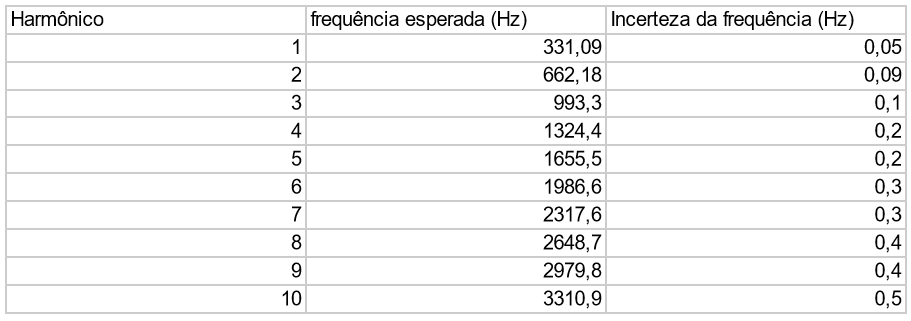
\includegraphics[scale=0.5]{harmonicos_1_incerteza.png}
    \caption{Tabela 1}
    \label{fig:Figura 1}
\end{figure}
\qquad Para o caso aberto-fechado e fechado-aberto utilizamos as relações anteriores, mas nesse caso $kL = \eta 2$ e obtivemos essa tabela para as frequências esperadas:

\begin{figure}[!htb]
    \centering
   % 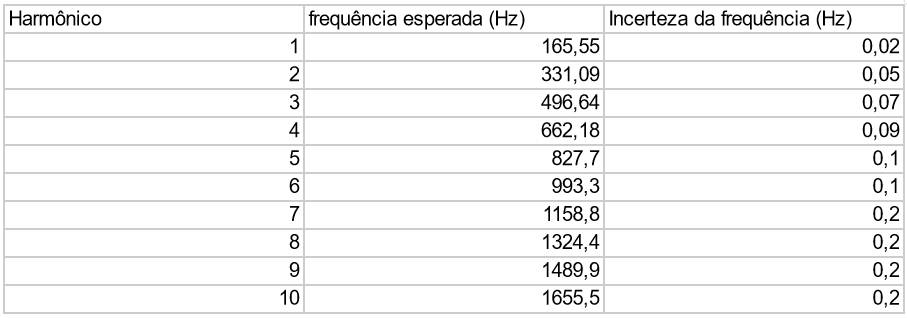
\includegraphics[scale=0.5]{harmonicos_2_incerteza.png}
    \caption{Tabela 2}
    \label{fig:Figura 1}
\end{figure}
\qquad Para os gráficos por hora conseguimos constatar o de amplitude da pressão pela frequência:
\begin{figure}[!htb]
    \centering
  %  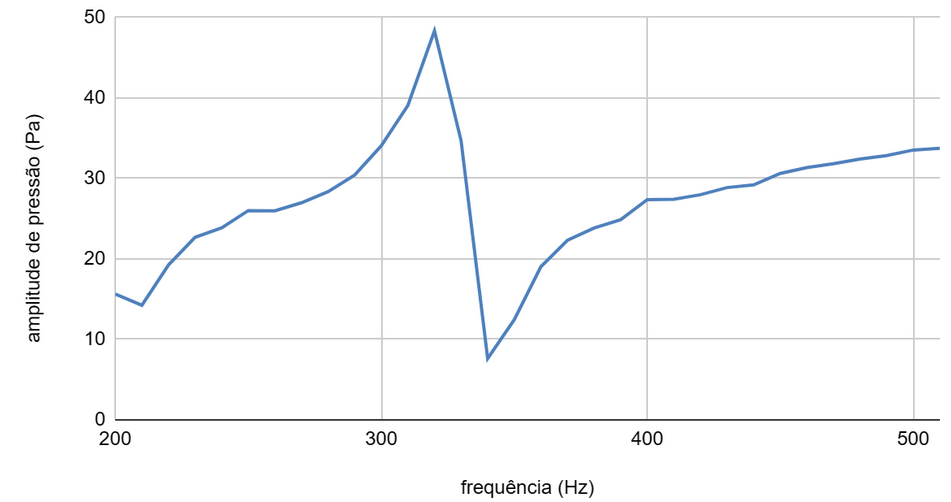
\includegraphics[scale=0.5]{diferencadepressao_porfrequencia_aberto_aberto.png}
    \caption{Diferença de Pressão pela frequência no tubo aberto-aberto}
    \label{fig:Figura 1}
\end{figure}
\qquad Podemos observar que próximo à frequência esperada de $346,19 Hz$ verificamos um ponto de máximo e um mínimo, algo que não esperávamos pela equação da pressão para um harmônico em um tubo aberto-aberto:
\begin{equation}
    Pe(x,t) = A \sin{(kx)}kx\cos{(\omega t)}
\end{equation}
\qquad Como colocamos o nosso microfone na posição $x = 0$, logo esperávamos que a pressão nessa posição fosse 0 quando ocorresse um harmônico. Mas como observado, a pressão não corresponde com os dados coletados, já que o ponto mais próximo de 0 possui o valor de $340 Hz$ que de acordo com o cálculo do tubo seria o valor do primeiro harmônico.
Utilizando a equação abaixo, podemos notar que a velocidade do som obtida no tubo aberto-aberto foi de: 
\begin{equation}
    \nu = \lambda f = \frac{2 L'}{\eta} f = 356 \pm 6 m/s
\end{equation}
\qquad A velocidade obtida acima está a menos de 2 desvios padrões da velocidade calculada pelo software $Wolfram Alpha$, onde constata-se o valor de $346,19 m/s$. O que não exclui o fato da incerteza atingir um valor muito alto, o que se faz necessário uma alternativa para minimizar esse fator. Uma possível solução seria diminuir os intervalos entre as frequências emitidas pelo software $Phyphox$.
Já para o caso aberto-fechado do tubo de PVC, capturamos o seguinte gráfico: 
\begin{figure}[!htb]
    \centering
  %  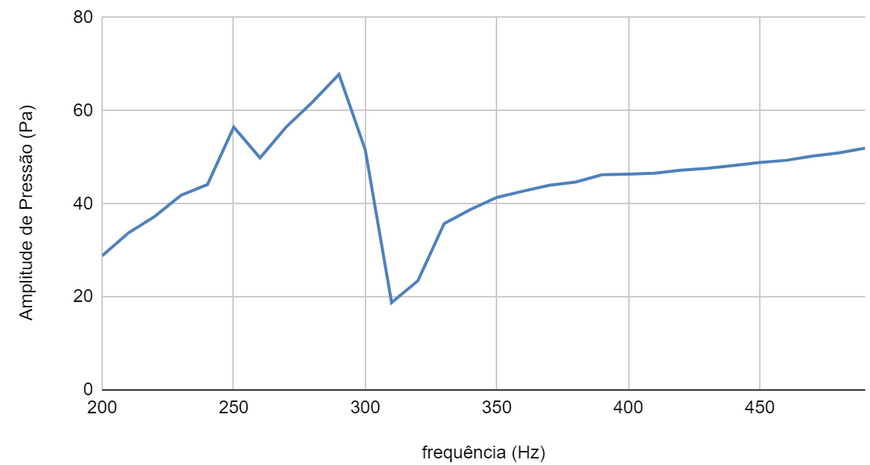
\includegraphics[scale=0.5]{pa_x_hz.png}
    \caption{Gráfico de amplitude de pressão $(Pa)$ versus frequência $(Hz)$ }
    \label{fig:enter-label}
\end{figure}
é observável que a frequência esperada 331,09 Hz está depois de um ponto de mínimo, algo que não esperávamos pela equação da pressão para um harmônico em um tubo aberto-aberto, como demosntrado a seguir:
\begin{equation}
    P_e(x,t) = A \sin{(kx)}\cos{(\omega t)}
\end{equation}
\qquad Utilizando a equação abaixo, a velocidade do som obtida no tubo aberto-fechado foi de: 
\begin{equation}
    \nu = \lambda f = \frac{2 L'}{\eta} f = 324 \pm 6 m/s
\end{equation}
\qquad No qual esse valor ficou a mais de 3 desvios padrões calculados pelo software $Wolfram Alpha$, onde observamos que ficou muito longe do previsto, o que se faz necessário uma nova análise.


\section*{Discussão}
\qquad Acreditamos que pelos dados coletados não conseguimos fazer uma análise rica e próxima da que está descrita no guia do experimento, já que no momento da coleta de dados erramos o procedimento o que se faz necessário uma nova bateria de coleta de dados e uma maneira mais sólida de coletar esses dados com o máximo de precisão possível.
\section*{Resultados}
\qquad Ainda faltam muitos resultados experimentais a serem analisados devido a coleta de dados.
\section*{Conclusão}
\qquad Como apontado na seção de discussão, não podemos e nem temos embasamento científico suficiente neste momento para concluir algo relevante ao experimento a não ser o fato de que necessitamos enriquecer a etapa da coleta de dados para tratarmos valores mais precisos e confiáveis.
\section*{Referências}
“F 229 — Física Experimental II, Guia de Laboratório”, Coordenador: Pierre-Louis de Assis, versão 1.1.0 (outubro 2022) \\ \ \\ 
\qquad Hollow Cylinder Moment of Inertia. Disponível em: https://amesweb.info/inertia/hollow-cylinder-moment-of-inertia.aspx\\ \ \\ 
NUSSENZVEIG, H. Moysés. Curso de física básica 2: Fluidos, oscilações e ondas, calor. 5.ed. São Paulo: Blucher, 2013.\\ \ \\

\section*{Apêndice A: Dados experimentais e incertezas}
\end{document}